\documentclass[border=0pt]{standalone}
\usepackage{amsmath,amssymb}
\usepackage{xcolor}
\usepackage{tikz}
\usetikzlibrary{arrows.meta,calc,decorations.pathreplacing,positioning,shapes.geometric,backgrounds}
\definecolor{c1}{RGB}{0,114,178}
\definecolor{c2}{RGB}{230,159,0}
\definecolor{c3}{RGB}{0,158,115}
\definecolor{cr}{RGB}{213,94,0}
\tikzset{every picture/.append style={show background rectangle,
    background rectangle/.style={fill=white}, inner frame sep=8pt}}
\newcommand{\roll}{\mathcal{R}}
\begin{document}
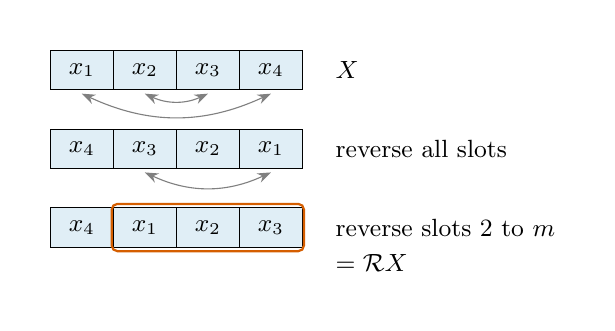
\begin{tikzpicture}[>=Stealth, box/.style={draw, minimum width=0.8cm, minimum height=0.5cm,
      fill=c1!12, font=\small}]
    \foreach \row/\a/\b/\c/\d/\lab in {0/x_1/x_2/x_3/x_4/{$X$},
                                      1/x_4/x_3/x_2/x_1/{reverse all slots},
                                      2/x_4/x_1/x_2/x_3/{reverse slots $2$ to $m$}} {
      \node[box] at (0, -1.0*\row) {$\a$};
      \node[box] at (0.8, -1.0*\row) {$\b$};
      \node[box] at (1.6, -1.0*\row) {$\c$};
      \node[box] at (2.4, -1.0*\row) {$\d$};
      \node[anchor=west, font=\small] at (3.1, -1.0*\row) {\lab};
    }
    \draw[<->, gray] (0, -0.3) to[bend right=25] (2.4, -0.3);
    \draw[<->, gray] (0.8, -0.3) to[bend right=25] (1.6, -0.3);
    \draw[<->, gray] (0.8, -1.3) to[bend right=25] (2.4, -1.3);
    \draw[thick, cr, rounded corners=2pt] (0.38, -2.3) rectangle (2.82, -1.7);
    \node[anchor=west, font=\small] at (3.1, -2.45) {$= \roll X$};
  \end{tikzpicture}
\end{document}
